%%%%%%%%%%%%%%%%%%%%%%%%%%%%%%%%%%%%%%%%%%%%%%%%%%%%%%%%%%%%%%%%%%%%%%%%%%%%%%%%%%%%
%%%   Copyright  2015  SRNS.RU Team                                              %%%
%%%      _______. .______     .__   __.      ___ ____.    .______      __    __  %%%
%%%     /       | |   _  \    |  \ |  |     /       |     |   _  \    |  |  |  | %%%
%%%    |   (----` |  |_)  |   |   \|  |    |   (----`     |  |_)  |   |  |  |  | %%%
%%%     \   \     |      /    |  . `  |     \   \         |      /    |  |  |  | %%%
%%% .----)   |    |  |\  \--. |  |\   | .----)   |    __  |  |\  \--. |  `--'  | %%%
%%% |_______/     | _| `.___| |__| \__| |_______/    (__) | _| `.___|  \______/  %%%
%%%                                                                              %%%
%%%   Boldenkov E., Korogodin I.                                                 %%%
%%%                                                                              %%%
%%%   Licensed under the Apache License, Version 2.0 (the "License");            %%%
%%%   you may not use this file except in compliance with the License.           %%%
%%%   You may obtain a copy of the License at                                    %%%
%%%                                                                              %%%
%%%       http://www.apache.org/licenses/LICENSE-2.0                             %%%
%%%                                                                              %%%
%%%   Unless required by applicable law or agreed to in writing, software        %%%
%%%   distributed under the License is distributed on an "AS IS" BASIS,          %%%
%%%   WITHOUT WARRANTIES OR CONDITIONS OF ANY KIND, either express or implied.   %%%
%%%   See the License for the specific language governing permissions and        %%%
%%%   limitations under the License.                                             %%%
%%%%%%%%%%%%%%%%%%%%%%%%%%%%%%%%%%%%%%%%%%%%%%%%%%%%%%%%%%%%%%%%%%%%%%%%%%%%%%%%%%%%

\section{Соглашения о терминологии и обозначениях}

В дальнейшем описании будем руководствоваться следующими принципами.

При описании алгоритмов функционирования устройств помимо математических формул будет испольльзоваться синтаксис языков C, Matlab, Verilog.

\textcolor{red}{Красным} цветом отмечено описание нереализованных функций, \textcolor{green}{зеленым} - те места документа, которые требуют доработки (чаще всего требуется словесное описание заменить таблицей).

\texttt{CRPA\_BASE} - базовый адрес регистровой памяти, относительно которого заданы смещения карты памяти

Все регистры являются 32-разрядными.

Управление доступом:
\begin{itemize}
\item[ro] -- только чтение
\item[wo] -- только запись
\item[rw] -- чтение/запись
\end{itemize}


%%%%%%%%%%%%%%%%%%%%%%%%%%%%%%%%%%%%%%%%%%%%%%%%%%%%%%%%%%%%%%%%%%%%%%%%%%%%%%%%%%%%%%%%%%%%%%%%%%%%%%%%%
\newpage
\section{Регистры блока пространственной обработки}
\label{sec:commons}

\subsection{Карта регистров блока пространственной обработки}
\begin{longtable}{|p{30mm}|p{55mm}|p{6cm}|p{15mm}|}
\hline
\textbf{Смещение, байт (слов)} & \textbf{Название} & \textbf{Описание} & \textbf{Раздел (cсылка)} \\
\hline
% 1 & 2 & 3 & 4  \\
% \hline\endfirsthead
% \hline
% 1 & 2 & 3 & 4 \\
% \hline\hline\endhead
% \hline
% \multicolumn{3}{c}{\textit{Продолжение на следующей странице}}
% \endfoot\hline\endlastfoot
\multicolumn{4}{|c|}{\textit{Управляющие регистры}} \\
\hline
0x00 (0x00)  & CRPA\_ID             	& Идентификатор блока пространственной обработки& \ref{sec:CRPA_ID} \\
\hline
0x04 (0x01)  & CRPA\_PARAMS   	        & Параметры блока пространственной обработки 	& \ref{sec:CRPA_PARAMS} \\
\hline
0x08 (0x02)  & CRPA\_CONTROL      	& Управление блоком пространственной обработки 	& \ref{sec:CRPA_CONTROL} \\
\hline
0x0C (0x03)  & CRPA\_STATUS    	        & Статус блока пространственной обработки 	& \ref{sec:CRPA_STATUS} \\
\hline
0x10 (0x04)  & CRPA\_IRQ\_RELEASE      	& Регистр количества накапливаемых отсчётов     & \ref{sec:CRPA_IRQ_RELEASE} \\
\hline
0x14 (0x05)  & CRPA\_MASTER         	& Регистр программного выбора master/slave      & \ref{sec:CRPA_MASTER} \\
\hline
\multicolumn{4}{|c|}{\textit{Тестовый генератор}} \\
\hline
0x18 (0x06)  & GEN\_CONTROL            	& Управление тестовым генератором               & \ref{sec:GEN_CONTROL} \\
\hline
0x1C (0x07)  & GEN\_PHASE\_RATE        	& Код частоты тестового сигнала                 & \ref{sec:GEN_PHASE_RATE} \\
\hline
0x20 (0x08)  & GEN\_SCALE            	& Амплитуда тестового сигнала                   & \ref{sec:GEN_SCALE} \\
\hline
0x24 (0x09)  & GEN\_CONST            	& Тестовая константа                            & \ref{sec:GEN_CONST} \\
\hline
\multicolumn{4}{|c|}{\textit{Мультиплексор}} \\
\hline
0x28 (0x0A)  & MUX1\_CONTROL           	& Выбор входа                                   & \ref{sec:MUX1_CONTROL} \\
\hline
% 0x2A (0x0B)  & MUX2\_CONTROL           	& Параметры мультиплексора                      & \ref{sec:MUX2_CONTROL} \\
% \hline
\multicolumn{4}{|c|}{\textit{FIFO}} \\
\hline
0x30 (0x0C)  & FIFO\_RESET           	& Сброс FIFO                                    & \ref{sec:FIFO_RESET} \\
\hline
\multicolumn{4}{|c|}{\textit{Управление тактовыми сигналами}} \\
\hline
0x38 (0x0E)  & CLK\_GATE\_CTRL        	& Регистр управления тактовыми сигналами        & \ref{sec:CLK_GATE_CTRL} \\
\hline
0x3C (0x0F)  & RST\_GATE\_CTRL        	& Регистр сброса                                & \ref{sec:RST_GATE_CTRL} \\
\hline


\multicolumn{4}{|c|}{\textit{Статус корреляционной матрицы}} \\
\hline
0x40 (0x10)  & CVM\_STATUS        	& Регистр статуса блока расчёта матрицы         & \ref{sec:CVM_STATUS} \\
\hline

\multicolumn{4}{|c|}{\textit{Параметры блока пространственной обработки}} \\
\hline
0x44 (0x11)  & DATA\_WIDTH0        	& Регистр разрядности внутренних данных         & \ref{sec:DATA_WIDTH0} \\
\hline
0x48 (0x12)  & DATA\_WIDTH1        	& Регистр разрядности внутренних данных         & \ref{sec:DATA_WIDTH1} \\
\hline

0x4C (0x13)  & NF\_ADDR          	& Смещение блока формирователя нулей            & \ref{sec:NF_ADDR} \\
\hline
0x50 (0x14)  & NF\_STEP          	& Размер канала формирователя нулей             & \ref{sec:NF_STEP} \\
\hline

0x54 (0x15)  & BF\_RE\_ADDR          	& Смещение действительных формирователей лучей  & \ref{sec:BF_RE_ADDR} \\
\hline
0x58 (0x16)  & BF\_IM\_ADDR          	& Смещение мнимых формирователей лучей          & \ref{sec:BF_IM_ADDR} \\
\hline
0x5C (0x17)  & BF\_STEP          	& Размер блока формирователей лучей             & \ref{sec:BF_STEP} \\
\hline

0x60 (0x18)  & CVM\_ADDR          	& Смещение блока расчёта матрицы                & \ref{sec:CVM_ADDR} \\
\hline
0x64 (0x19)  & CVM\_LENGTH          	& Размер блока корреляционной матрицы           & \ref{sec:CVM_LENGTH} \\
\hline
0x68 (0x1A)  & CVM\_TYPEDESCR0         	& Описание структуры корреляционной матрицы     & \ref{sec:CVM_TYPEDESCR0} \\
\hline
0x6C (0x1B)  & CVM\_TYPEDESCR1         	& Описание структуры корреляционной матрицы     & \ref{sec:CVM_TYPEDESCR1} \\
\hline

\multicolumn{4}{|c|}{\textit{Флаги правильных данных}} \\
\hline

0x70 (0x1C)  & VALID\_NF          	& Флаги правильных данных формирователя нулей   & \ref{sec:VALID_NF} \\
\hline
0x74 (0x1D)  & VALID\_BF          	& Флаги правильных данных формирователя лучей   & \ref{sec:VALID_BF} \\
\hline
0x78 (0x1E)  & VALID\_SIGMAG          	& Флаги правильных данных блока квантования     & \ref{sec:VALID_SIGMAG} \\
\hline

\multicolumn{4}{|c|}{\textit{Регистры блоков помехоподавления}} \\
\hline
\tiny NF\_ADDR+NF\_STEP*1 & CRPA\_NF\_0      	& Регистры помехоподавителя 0 			& \ref{sec:CRPA_NF} \\
\hline
\tiny NF\_ADDR+NF\_STEP*1 & CRPA\_NF\_1      	& Регистры помехоподавителя 1 		        & \ref{sec:CRPA_NF} \\
\hline
\multicolumn{4}{|c|}{...} \\
\hline
\tiny NF\_ADDR+NF\_STEP*7 & CRPA\_NF\_7      	& Регистры помехоподавителя 7 		        & \ref{sec:CRPA_NF} \\
\hline
\multicolumn{4}{|c|}{\textit{Регистры блоков фокусировки}} \\
\hline
\tiny BF\_RE\_ADDR+BF\_STEP*0  & CRPA\_BF\_RE\_0  & Регистры блока фокусировки 0 		& \ref{sec:CRPA_BF} \\
\hline
\tiny BF\_RE\_ADDR+BF\_STEP*1  & CRPA\_BF\_RE\_1  & Регистры блока фокусировки 1 		& \ref{sec:CRPA_BF} \\
\hline
\multicolumn{4}{|c|}{...} \\
\hline
\tiny BF\_RE\_ADDR+BF\_STEP*11 & CRPA\_BF\_RE\_11 & Регистры блока фокусировки 11		& \ref{sec:CRPA_BF} \\
\hline
\tiny BF\_IM\_ADDR+BF\_STEP*0  & CRPA\_BF\_IM\_0  & Регистры блока фокусировки 0 		& \ref{sec:CRPA_BF} \\
\hline
\tiny BF\_IM\_ADDR+BF\_STEP*1  & CRPA\_BF\_IM\_1  & Регистры блока фокусировки 1 		& \ref{sec:CRPA_BF} \\
\hline
\multicolumn{4}{|c|}{...} \\
\hline
\tiny BF\_IM\_ADDR+BF\_STEP*11 & CRPA\_BF\_IM\_11 & Регистры блока фокусировки 11		& \ref{sec:CRPA_BF} \\
\hline
\multicolumn{4}{|c|}{\textit{Регистры блока расчёта корреляционной матрицы}} \\
\hline
\tiny CVM\_ADDR    & CRPA\_CM         	& Регистры блока расчёта корреляционной матрицы & \ref{sec:CRPA_CM} \\
\hline
\end{longtable}


\subsection{Управляющие регистры}

\subsubsection{CRPA\_ID~ (0x00)}
\renewcommand{\regnam}{CRPA\_ID~}
\label{sec:CRPA_ID}

\begin{register}{H}{Идентификатор блока пространственной обработки \regnam}{0x00}
\label{reginterruptcontrol}%
\regfield{ID}{16}{16}{{0xAE13}}%
\regfield{reserved}{16}{0}{{xxxxxxxxxxxxxxxx}}%
\reglabel{По сбросу}
\regnewline%

\begin{regdesc}\begin{reglist}
\item [ID (ro)]
Идентификация начала блока регистров управления импульсом прерывания.
\item [reserved (ro)]
Зарезервированные биты.
\end{reglist}\end{regdesc}
\end{register}


\subsubsection{CRPA\_PARAMS~ (0x04)}
\renewcommand{\regnam}{CRPA\_PARAMS~}
\label{sec:CRPA_PARAMS}

\begin{register}{H}{Регистр параметров блока пространственной обработки \regnam}{0x04}
\label{reginterruptperiod}%
\regfield{Reserved}{12}{20}{{0x000}}%
\regfield{MASTER\_SLAVE}{4}{16}{{0x0}}%
\regfield{NNF}{4}{12}{{0x0}}%
\regfield{NBF}{4}{8}{{0x0}}%
\regfield{NCH}{4}{4}{{0x0}}%
\regfield{NT}{4}{0}{{0x0}}%
\reglabel{По сбросу}
\regnewline%

\begin{regdesc}\begin{reglist}
\item [NT (ro)]
Количество отводов по времени в пространственно-временном фильтре помехоподавления.
\item [NCH (ro)]
Количество пространственных входов в пространственно-временном фильтре помехоподавителя.
\item [NBF (ro)]
Количество блоков формирования лучей.
\item [NNF (ro)]
Количество блоков формирования нулей.
\item [MASTER\_SLAVE (ro)]
Копия состояния Master/slave.
\item [Reserved]
Зарезервированные биты.
\end{reglist}\end{regdesc}
\end{register}


\subsubsection{CRPA\_CONTROL~ (0x08)}
\renewcommand{\regnam}{CRPA\_CONTROL~}
\label{sec:CRPA_CONTROL}

\begin{register}{H}{Регистр управления блоком пространственной обработки \regnam}{0x08}
\label{reginterruptduration}%
\regfield{NF\_LOAD\_EN}{1}{31}{{0x0}}%
\regfield{CVM\_LOAD\_EN}{1}{30}{{0x0}}%
\regfield{Reserved}{4}{26}{{0x000000}}%
\regfield{CVM\_mode}{2}{24}{{0x0}}%
\regfield{CVM\_Nstat}{12}{6}{{1024}}%
\regfield{NF\_start}{1}{4}{{0x0}}%
\regfield{CVM\_start}{1}{3}{{0x0}}%
\regfield{Reserved}{2}{0}{{0x0}}%
\reglabel{По сбросу}
\regnewline%

\begin{regdesc}\begin{reglist}
\item [CVM\_start (rw)]
Сигнал запуска сбора корреляционной матрицы
Для запуска надо записать ``1'', для сброса записать ``0''.
\item [CRPA\_NF\_start (rw)]
Сигнал загрузки коэфициентов; \\
\item [CVM\_mode (rw)]
Тип корреляционной матрицы; \\  
\item [CVM\_LOAD\_EN (rw)]
Флаг разрешения внешнего сигнала запуска сбора корреляционной матрицы; \\
\item [NF\_LOAD\_EN (rw)]
Флаг разрешения внешнего сигнала загрузки коэффициентов пространственно-временных фильтров \\
\end{reglist}\end{regdesc}
\end{register}


\subsubsection{CRPA\_STATUS~ (0x0C)}
\renewcommand{\regnam}{CRPA\_STATUS~}
\label{sec:CRPA_STATUS}

\begin{register}{H}{Регистр статуста блока пространственной обработки \regnam}{0x0A}
\label{regsamplecount}%
\regfield{Reserved}{31}{1}{{0x00000000}}%
\regfield{CVM\_READY}{1}{0}{{0x0}}%
\reglabel{Имя (По сбросу)}\regnewline%

\begin{regdesc}\begin{reglist}
\item [CVM\_READY (r)]
Флаг готовности результата накопления корреляционной матрицы.
\item [Reserved]
Зарезервированные биты
\end{reglist}\end{regdesc}
\end{register}

\subsubsection{CRPA\_IRQ\_RELEASE~ (0x10)}
\renewcommand{\regnam}{CRPA\_IRQ\_RELEASE~}
\label{sec:CRPA_IRQ_RELEASE}

\begin{register}{H}{Регистр сброса прерывания \regnam}{0x10}
\label{regsamplecount}%
\regfield{Reserved}{32}{0}{{0x0}}%
\reglabel{Имя (По сбросу)}\regnewline%

\begin{regdesc}\begin{reglist}
\item [Reserved (rw)]
Запись любого значения сбрасывает прерывание
\end{reglist}\end{regdesc}
\end{register}

\subsubsection{CRPA\_MASTER~ (0x14)}
\renewcommand{\regnam}{CRPA\_MASTER~}
\label{sec:CRPA_MASTER}

\begin{register}{H}{Регистр управления режимом синхронизации Master/slave \regnam}{0x0C}
\label{regsamplecount}%
\regfield{Reserved}{31}{1}{{0x00000000}}%
\regfield{CRPA\_MASTER}{1}{0}{{X}}%
\reglabel{Имя (По сбросу)}\regnewline%

\begin{regdesc}\begin{reglist}
\item [CRPA\_MASTER (rw)]
Бит управления режимом синхронизации master/slave. Начальное значение определяется
состоянием вывода Master/slave в момент сброса.
\end{reglist}\end{regdesc}
\end{register}

\subsection{Регистры управления тестовым генератором}

\subsubsection{GEN\_CONTROL~ (0x18)}
\renewcommand{\regnam}{GEN\_CONTROL~}
\label{sec:GEN_CONTROL}

\begin{register}{H}{Регистр управления режимом тестового генератора \regnam}{0x18}
\label{regsamplecount}%
\regfield{Reserved}{21}{11}{{0x00000000}}%
\regfield{GEN\_CH\_DISABLE}{8}{3}{{0x0}}%
\regfield{GEN\_ENABLE}{1}{2}{{0x0}}%
\regfield{SIGNAL\_TYPE}{1}{1}{{0x0}}%
\regfield{SYNC\_RESET}{1}{0}{{0x0}}%
\reglabel{Имя (По сбросу)}\regnewline%

\begin{regdesc}\begin{reglist}
\item [SYNC\_RESET (rw)]
Синхронный сброс (активный уровень 1).
\item [SIGNAL\_TYPE (rw)]
Выбор типа тестового сигнала (0 - синус, 1 - константа).
\item [GEN\_ENABLE (rw)]
Разрешение работы тестового генератора (активный уровень 1).
\item [GEN\_CH\_DISABLE (rw)]
Отдельное отключение каналов тестового генератора.
\item [Reserved]
Зарезервированные биты.
\end{reglist}\end{regdesc}
\end{register}

\subsubsection{GEN\_PHASE\_RATE~ (0x1C)}
\renewcommand{\regnam}{GEN\_PHASE\_RATE~}
\label{sec:GEN_PHASE_RATE}

\begin{register}{H}{Регистр частоты тестового сигнала \regnam}{0x1C}
\label{regsamplecount}%
\regfield{PHASE\_RATE}{32}{0}{{0x0}}%
\reglabel{Имя (По сбросу)}\regnewline%

\begin{regdesc}\begin{reglist}
\item [PHASE\_RATE (rw)]
Код частоты опорного сигнала.
\end{reglist}\end{regdesc}
\end{register}

Тестовый сигнал представляет собой синусоиду, формируемую методом прямого цифрового
синтеза по таблице. Разрядность таблицы по фазе 5 разрядов, по амплитуде - 4 разряда.
Частота тестового сигнала определяется выражением:
\[
   f = \frac{PHASE\_RATE}{2^{32}}\cdot f_{CLK}
\]


\subsubsection{GEN\_SCALE~ (0x20)}
\renewcommand{\regnam}{GEN\_SCALE~}
\label{sec:GEN_SCALE}

\begin{register}{H}{Регистр управления амплитудой тестового генератора \regnam}{0x20}
\label{regsamplecount}%
\regfield{Reserved}{27}{5}{{0x000000}}%
\regfield{SCALE}{5}{0}{{0x0}}%
\reglabel{Имя (По сбросу)}\regnewline%

\begin{regdesc}\begin{reglist}
\item [SCALE (rw)]
Масштабный коэффициент.
\item [Reserved]
Зарезервированные биты.
\end{reglist}\end{regdesc}
\end{register}

Разрядность сигнала на выходе тестового генератора --- 4 разряда. Разрядность линии данных
--- 16. Коэффициент SCALE определяет, на сколько разрядов влево сдвигается значение на
выходе тестового генератора перед подачей на линию данных.

\subsubsection{GEN\_CONST~ (0x24)}
\renewcommand{\regnam}{GEN\_CONST~}
\label{sec:GEN_CONST}

\begin{register}{H}{Регистр тестовой константы \regnam}{0x24}
\label{regsamplecount}%
\regfield{CONST}{32}{0}{{0x0}}%
\reglabel{Имя (По сбросу)}\regnewline%

\begin{regdesc}\begin{reglist}
\item [CONST (rw)]
Тестовая константа.
\end{reglist}\end{regdesc}
\end{register}

\subsection{Регистры управления мультиплексором}

\subsubsection{MUX1\_CONTROL~ (0x28)}
\renewcommand{\regnam}{MUX1\_CONTROL~}
\label{sec:MUX1_CONTROL}

\begin{register}{H}{Выбор входа \regnam}{0x28}
\label{regsamplecount}%
\regfield{Reserved}{31}{1}{{0x00000000}}%
\regfield{SELECT}{1}{0}{{0x0}}%
\reglabel{Имя (По сбросу)}\regnewline%

\begin{regdesc}\begin{reglist}
\item [SELECT (rw)]
Выбор сигнала (0 --- АЦП, 1 --- тестовый сигнал).
\item [Reserved]
Зарезервированные биты.
\end{reglist}\end{regdesc}
\end{register}

% \subsubsection{MUX2\_CONTROL~ (0x2C)}
% \renewcommand{\regnam}{MUX2\_CONTROL~}
% \label{sec:MUX2_CONTROL}

% \begin{register}{H}{Параметры мультиплексора \regnam}{0x2C}
% \label{regsamplecount}%
% \regfield{Reserved}{29}{3}{{0x00000000}}%
% \regfield{MUX2\_resetn\_sigmag}{1}{2}{{0x0}}%
% \regfield{MUX2\_resetn\_mean}{1}{1}{{0x0}}%
% \regfield{MUX2\_mean\_en}{1}{0}{{0x0}}%
% \reglabel{Имя (По сбросу)}\regnewline%

% \begin{regdesc}\begin{reglist}
% \item [MUX2\_mean\_en (rw)]
% Разрешение блока компенсации постоянного смещения.
% \item [MUX2\_resetn\_mean (rw)]
% Сброс блока расчёта математического ожидания.
% \item [MUX2\_resetn\_sigmag (rw)]
% Сброс блока адаптации порогов двухуровневого квантователя.
% \item [Reserved]
% Зарезервированные биты.
% \end{reglist}\end{regdesc}
% \end{register}

\subsection{Регистры управления FIFO}

\subsubsection{FIFO\_RESET~ (0x30)}
\renewcommand{\regnam}{FIFO\_RESET~}
\label{sec:FIFO_RESET}

\begin{register}{H}{Выбор входа \regnam}{0x30}

\label{regsamplecount}%
\regfield{Reserved}{31}{1}{{0x00000000}}%
\regfield{FIFO\_RESET}{1}{0}{{0x0}}%
\reglabel{Имя (По сбросу)}\regnewline%

\begin{regdesc}\begin{reglist}
\item [FIFO\_RESET (rw)]
Сброс FIFO (активный уровень 1).
\item [Reserved]
Зарезервированные биты.
\end{reglist}\end{regdesc}
\end{register}

\subsection{Управление тактовыми сигналами}

\subsubsection{CLK\_GATE\_CTRL~ (0x38)}
\renewcommand{\regnam}{CLK\_GATE\_CTRL~}
\label{sec:CLK_GATE_CTRL}

\begin{register}{H}{Включение тактовых сигналов отдельных блоков \regnam}{0x38}

\label{regsamplecount}%
\regfield{Reserved}{25}{6}{{0x0000000}}%
\regfield{DCOL\_CLK}{1}{5}{{0}}%
\regfield{BF\_CLK}{2}{3}{{00}}%
\regfield{NF\_CLK}{2}{1}{{00}}%
\regfield{CVM\_CLK}{1}{0}{{0}}%
\reglabel{Имя (По сбросу)}\regnewline%

\begin{regdesc}\begin{reglist}
\item [DCOL\_CLK (rw)]
Управление тактовым сигналом блока сбора данных (1 - включить).
\item [BF\_CLK (rw)]
Управление тактовыми сигналами блоков формирователей лучей (0 --- выключить, 1 ---
включить блок 0, 2 --- включить блоки 1-11, 3 --- включить все блоки).
\item [NF\_CLK (rw)]
Управление тактовыми сигналами блоков формирователей нулей (0 --- выключить, 1 ---
включить блок 0, 2 --- включить блоки 1-7, 3 --- включить все блоки).
\item [CVM\_CLK (rw)]
Управление тактовым сигналом блока накопления корреляционной матрицы (1 - включить).
\item [Reserved]
Зарезервированные биты.
\end{reglist}\end{regdesc}
\end{register}

\subsubsection{RST\_GATE\_CTRL~ (0x3C)}
\renewcommand{\regnam}{RST\_GATE\_CTRL~}
\label{sec:RST_GATE_CTRL}

\begin{register}{H}{Выбор входа \regnam}{0x3C}

\label{regsamplecount}%
\regfield{Reserved}{25}{6}{{0x0000000}}%
\regfield{DCOL\_RST}{1}{5}{{0}}%
\regfield{BF\_RST}{2}{3}{{00}}%
\regfield{NF\_RST}{2}{1}{{00}}%
\regfield{CVM\_RST}{1}{0}{{0}}%
\reglabel{Имя (По сбросу)}\regnewline%

\begin{regdesc}\begin{reglist}
\item [DCOL\_CLK (rw)]
Сброс блока сбора данных (активный низкий).
\item [BF\_CLK (rw)]
Сброс блоков формирователей лучей (0 --- сброс всех, 1 ---
сброс блоков 1-11, 2 --- сброс блока 0, 3 --- включить все блоки).
\item [NF\_CLK (rw)]
Сброс блоков формирователей нулей (0 --- сброс всех, 1 ---
сброс блоков 1-7, 2 --- сброс блока 0, 3 --- включить все блоки).
\item [CVM\_CLK (rw)]
Сброс блока накопления корреляционной матрицы (активный низкий).
\item [Reserved]
Зарезервированные биты.
\end{reglist}\end{regdesc}
\end{register}


\subsection{Статус корреляционной матрицы}

\subsubsection{CVM\_STATUS~ (0x40)}
\renewcommand{\regnam}{CVM\_STATUS~}
\label{sec:CVM_STATUS}

\begin{register}{H}{Статус блока расчёта корреляционной матрицы \regnam}{0x40}

\label{regsamplecount}%
\regfield{Reserved}{31}{1}{{0x00000000}}%
\regfield{CVM\_STATUS}{1}{0}{{0x0}}%
\reglabel{Имя (По сбросу)}\regnewline%

\begin{regdesc}\begin{reglist}
\item [CVM\_STATUS (rw)]
Статус корреляционной матрицы (1 --- вычисление завершено).
\item [Reserved]
Зарезервированные биты.
\end{reglist}\end{regdesc}
\end{register}

\subsection{Параметры блока корреляционной обработки}

\subsubsection{DATA\_WIDTH0~ (0x44)}
\renewcommand{\regnam}{DATA\_WIDTH0~}
\label{sec:DATA_WIDTH0}

\begin{register}{H}{Разрядность внутреннего представления данных \regnam}{0x44}

\label{regsamplecount}%
\regfield{NF\_lsb\_drop}{8}{24}{{16}}%
\regfield{BF\_coeff\_width}{8}{16}{{16}}%
\regfield{NF\_coeff\_width}{8}{8}{{16}}%
\regfield{input\_width}{8}{0}{{16}}%
\reglabel{Имя (По сбросу)}\regnewline%

\begin{regdesc}\begin{reglist}
\item [NF\_lsb\_drop (r)]
Количество разрядов, отбрасываемых после блоков формирования лучей.
\item [BF\_coeff\_width (r)]
Разрядность коэффициентов блоков формирования лучей.
\item [NF\_coeff\_width (r)]
Разрядность коэффициентов блоков формирования нулей.
\item [input\_width (r)]
Разрядность входных данных.
\end{reglist}\end{regdesc}
\end{register}

\subsubsection{DATA\_WIDTH1~ (0x48)}
\renewcommand{\regnam}{DATA\_WIDTH1~}
\label{sec:DATA_WIDTH1}

\begin{register}{H}{Выбор входа \regnam}{0x48}

\label{regsamplecount}%
\regfield{CVM\_in\_width}{8}{24}{{14}}%
\regfield{CVM\_accum\_num}{8}{16}{{54}}%
\regfield{CVM\_accum\_width}{8}{8}{{42}}%
\regfield{BF\_out\_width}{8}{0}{{16}}%
\reglabel{Имя (По сбросу)}\regnewline%

\begin{regdesc}\begin{reglist}
\item [CVM\_in\_width (r)]
Входная разрядность блока расчёта корреляционной матрицы.
\item [CVM\_accum\_num (r)]
Количество накопителей блока расчёта корреляционной матрицы.
\item [CVM\_accum\_width (r)]
Разрядность накопителя блока расчёта корреляционной матрицы.
\item [BF\_out\_width (r)]
Выходная разрядность блоков формирования лучей
\end{reglist}\end{regdesc}
\end{register}

\subsubsection{NF\_ADDR~ (0x4C)}
\renewcommand{\regnam}{NF\_ADDR~}
\label{sec:NF_ADDR}

\begin{register}{H}{Начальный адрес коэффициентов формирователя нулей \regnam}{0x4C}

\label{regsamplecount}%
\regfield{NF\_ADDR}{32}{0}{{0x400}}%
\reglabel{Имя (По сбросу)}\regnewline%

\begin{regdesc}\begin{reglist}
\item [NF\_ADDR (rw)]
Начальный адрес коэффициентов блока 0 формирователя нулей относительно базового адреса
CRPA (байты).
\end{reglist}\end{regdesc}
\end{register}

\subsubsection{NF\_STEP~ (0x50)}
\renewcommand{\regnam}{NF\_STEP~}
\label{sec:NF_STEP}

\begin{register}{H}{Приращение адреса между каналами блока формирователя нулей \regnam}{0x50}

\label{regsamplecount}%
\regfield{NF\_STEP}{32}{0}{{32}}%
\reglabel{Имя (По сбросу)}\regnewline%

\begin{regdesc}\begin{reglist}
\item [NF\_STEP (rw)]
Приращение адреса между каналам блока формирователя нулей (слов).
\end{reglist}\end{regdesc}
\end{register}


\subsubsection{BF\_RE\_ADDR~ (0x54)}
\renewcommand{\regnam}{BF\_RE\_ADDR~}
\label{sec:BF_RE_ADDR}

\begin{register}{H}{Начальный адрес действительных коэффициентов формирователя лучей \regnam}{0x54}

\label{regsamplecount}%
\regfield{BF\_RE\_ADDR}{32}{0}{{0x4000}}%
\reglabel{Имя (По сбросу)}\regnewline%

\begin{regdesc}\begin{reglist}
\item [BF\_RE\_ADDR (rw)]
Начальный адрес действительных коэффициентов 0 формирователя лучей относительно базового
адреса CRPA (байты).
\end{reglist}\end{regdesc}
\end{register}

\subsubsection{BF\_IM\_ADDR~ (0x58)}
\renewcommand{\regnam}{BF\_IM\_ADDR~}
\label{sec:BF_IM_ADDR}

\begin{register}{H}{Начальный адрес мнимых коэффициентов формирователей лучей \regnam}{0x58}

\label{regsamplecount}%
\regfield{BF\_IM\_ADDR}{32}{0}{{0x4800}}%
\reglabel{Имя (По сбросу)}\regnewline%

\begin{regdesc}\begin{reglist}
\item [BF\_IM\_ADDR (rw)]
Начальный адрес мнимых коэффициентов 0 формирователя лучей относительно базового адреса
CRPA (байты).
\end{reglist}\end{regdesc}
\end{register}

\subsubsection{BF\_STEP~ (0x5C)}
\renewcommand{\regnam}{BF\_STEP~}
\label{sec:BF_STEP}

\begin{register}{H}{Приращение адреса между каналами блока формирователей лучей \regnam}{0x5C}

\label{regsamplecount}%
\regfield{BF\_STEP}{32}{0}{{8}}%
\reglabel{Имя (По сбросу)}\regnewline%

\begin{regdesc}\begin{reglist}
\item [BF\_STEP (rw)]
Приращение адреса между каналами блока формирователей лучей (слов).
\end{reglist}\end{regdesc}
\end{register}

\subsubsection{CVM\_ADDR~ (0x60)}
\renewcommand{\regnam}{CVM\_ADDR~}
\label{sec:CVM_ADDR}

\begin{register}{H}{Начальный адрес блока расчёта корреляционной матрицы \regnam}{0x60}

  \label{regsamplecount}%
  \regfield{CVM\_ADDR}{32}{0}{{0x5000}}%
  \reglabel{Имя (По сбросу)}\regnewline%

  \begin{regdesc}\begin{reglist}
    \item [CVM\_ADDR (rw)]
      Начальный адрес блока расчёта корреляционной матрицы относительно базового адреса
      CRPA (байты).
    \end{reglist}\end{regdesc}
\end{register}

\subsubsection{CVM\_LENGTH~ (0x64)}
\renewcommand{\regnam}{CVM\_LENGTH~}
\label{sec:CVM_LENGTH}

\begin{register}{H}{Количество элементов корреляционной матрицы \regnam}{0x64}

\label{regsamplecount}%
\regfield{CVM\_LENGTH}{32}{0}{{54}}%
\reglabel{Имя (По сбросу)}\regnewline%

\begin{regdesc}\begin{reglist}
\item [CVM\_LENGTH (r)]
Количество элементов корреляционной матрицы (слов).
\end{reglist}\end{regdesc}
\end{register}

\subsubsection{CVM\_TYPEDESCR0~ (0x68)}
\renewcommand{\regnam}{CVM\_TYPEDESCR0~}
\label{sec:CVM_TYPEDESCR0}

\begin{register}{H}{Конфигурация корреляционной матрицы \regnam}{0x68}

\label{regsamplecount}%
\regfield{INTCNT1}{16}{0}{{0x2109}}%
\regfield{INTCNT0}{16}{0}{{0x2009}}%
\reglabel{Имя (По сбросу)}\regnewline%

\begin{regdesc}\begin{reglist}
\item [INTCNT1 (r)]
Конфигурация корреляционной матрицы в режиме 1.
\item [INTCNT0 (r)]
Конфигурация корреляционной матрицы в режиме 0.
\end{reglist}\end{regdesc}
\end{register}

\subsubsection{CVM\_TYPEDESCR1~ (0x6C)}
\renewcommand{\regnam}{CVM\_TYPEDESCR1~}
\label{sec:CVM_TYPEDESCR1}

\begin{register}{H}{Конфигурация корреляционной матрицы \regnam}{0x6C}

\label{regsamplecount}%
\regfield{INTCNT3}{16}{0}{{0x0000}}%
\regfield{INTCNT2}{16}{0}{{0x0810}}%
\reglabel{Имя (По сбросу)}\regnewline%

\begin{regdesc}\begin{reglist}
\item [INTCNT3 (r)]
Конфигурация корреляционной матрицы в режиме 3.
\item [INTCNT2 (r)]
Конфигурация корреляционной матрицы в режиме 2.
\end{reglist}\end{regdesc}
\end{register}

\subsection{Флаги правильных данных}

\subsubsection{VALID\_NF~ (0x70)}
\renewcommand{\regnam}{VALID\_NF~}
\label{sec:VALID_NF}

\begin{register}{H}{Флаги правильных данных на выходах формирователей нулей \regnam}{0x70}

\label{regsamplecount}%
\regfield{Reserved}{24}{8}{{0x000000}}%
\regfield{VALID\_NF}{8}{0}{{0x00}}%
\reglabel{Имя (По сбросу)}\regnewline%

\begin{regdesc}\begin{reglist}
\item [VALID\_NF (rw)]
Флаги правильных данных на выходе каждого из блоков формирователя нулей (1 --- данные правильные).
\item [Reserved]
Зарезервированные биты.
\end{reglist}\end{regdesc}
\end{register}

\subsubsection{VALID\_BF~ (0x74)}
\renewcommand{\regnam}{VALID\_BF~}
\label{sec:VALID_BF}

\begin{register}{H}{Флаги правильных данных на выходах формирователей лучей \regnam}{0x74}

\label{regsamplecount}%
\regfield{Reserved}{20}{12}{{0x00000000}}%
\regfield{VALID\_BF}{12}{0}{{0x000}}%
\reglabel{Имя (По сбросу)}\regnewline%

\begin{regdesc}\begin{reglist}
\item [VALID\_BF (rw)]
Флаги правильных данных на выходах формирователей лучей (1 --- правильные данные).
\item [Reserved]
Зарезервированные биты.
\end{reglist}\end{regdesc}
\end{register}

\subsubsection{VALID\_SIGMAG~ (0x78)}
\renewcommand{\regnam}{VALID\_SIGMAG~}
\label{sec:VALID_SIGMAG}

\begin{register}{H}{Флаги правильных данных на выходах квантователей \regnam}{0x78}

\label{regsamplecount}%
\regfield{Reserved}{20}{12}{{0x00000000}}%
\regfield{VALID\_SIGMAG}{12}{0}{{0x000}}%
\reglabel{Имя (По сбросу)}\regnewline%

\begin{regdesc}\begin{reglist}
\item [VALID\_SIGMAG (rw)]
Флаги правильных данных на выходах блоков квантования (1 --- правильные данные).
\item [Reserved]
Зарезервированные биты.
\end{reglist}\end{regdesc}
\end{register}


\subsection{Регистры блоков помехоподавления}
\label{sec:CRPA_NF}

Смещения указаны относительно начального адреса блока помехоподавления
\texttt{CRPA\_NF\_x} (см. разд. \ref{sec:commons}).

Расположение коэффициентов зависит от параметров реализованного фильтра
(см. \ref{sec:CRPA_PARAMS}): NF\_TIME --- количества отводов по времени и NF\_CHAN ---
количества входов блока помехоподавления.

Каждый коэффициент представляет собой действительное целое число со знаком.

При записи новых коэффициентов по данным адресам происходит запись в теневые
регистры. Новые значения коэффициентов начинают использоваться после сигнала обновления
CRPA\_NF\_START, см. разд. \ref{sec:CRPA_CONTROL}.

\begin{longtable}{|c|p{3cm}|p{5cm}|p{3cm}|}
\hline
\textbf{Смещение} & \textbf{Название} & \textbf{Описание} & \textbf{Примечание} \\
% \hline
% 1 & 2 & 3 & 4  \\
% \hline\endfirsthead
% \hline
% 1 & 2 & 3 & 4 \\
% \hline\hline\endhead
% \hline
% \multicolumn{3}{c}{\textit{Продолжение на следующей странице}}
% \endfoot\hline\endlastfoot
\hline
0x00 (0x00) & CRPA\_NF\_K\_0\_0  & Коэффициент для 0 входа и 0 отвода по времени &  \\
\hline
0x04 (0x01) & CRPA\_NF\_K\_0\_1  & Коэффициент для 0 входа и 1 отвода по времени &  \\
\hline
\multicolumn{4}{|l|}{...} \\
\hline
0xXX (0xYY) & CRPA\_NF\_K\_I\_J  & Коэффициент для I входа и J отвода по времени & смещение
$4\times(I\cdot NF\_TIME + J)$ \\
\hline
\multicolumn{4}{|l|}{...} \\
\hline
0x7C  & CRPA\_NF\_K\_7\_3  & Коэффициент для 7 входа и 3 отвода по времени & при $NF\_TIME=4$ \\
\hline
\end{longtable}

\subsection{Регистры блоков фокусировки}
\label{sec:CRPA_BF}

Смещения указаны относительно начального адреса блока фокусировки
\texttt{CRPA\_BF\_x} (см. разд. \ref{sec:commons}).

Расположение коэффициентов зависит от параметров реализованного фильтра
(см. \ref{sec:CRPA_PARAMS}): NF\_TIME --- количества отводов по времени и NF\_CHAN ---
количества входов блока помехоподавления.

Каждый коэффициент представляет собой действительное целое число со знаком.

При записи новых коэффициентов в по данным адресам происходит запись в теневые
регистры. Новые значения коэффициентов начинают использоваться после сигнала обновления
CRPA\_BF\_START, см. разд. \ref{sec:CRPA_CONTROL}.

\begin{longtable}{|c|p{3cm}|p{5cm}|p{3cm}|}
\hline
\textbf{Смещение} & \textbf{Название} & \textbf{Описание} & \textbf{Примечание} \\
% \hline
% 1 & 2 & 3 & 4  \\
% \hline\endfirsthead
% \hline
% 1 & 2 & 3 & 4 \\
% \hline\hline\endhead
% \hline
% \multicolumn{3}{c}{\textit{Продолжение на следующей странице}}
% \endfoot\hline\endlastfoot
\hline
0x00 (0x00)  & CRPA\_BF\_RE\_K\_0  & Коэффициент для 0 входа &  \\
\hline
0x04 (0x01) & CRPA\_BF\_RE\_K\_0  & Коэффициент для 1 входа &  \\
\hline
\multicolumn{4}{|l|}{...} \\
\hline
0x20 (0x08) & CRPA\_BF\_K\_7  & Коэффициент для 7 входа &  \\
\hline
\end{longtable}

\subsection{Регистры блока расчёта корреляционной матрицы}
\label{sec:CRPA_CM}

Для вычисления коэффициентов фильтров пространственного подавления помех рассчитывается
матрица корреляционных коэффициентов.

Для расчёта матрицы формируется вектор задержанных отсчётов входного сигнала, имеющий вид,
приведённый на рис.~\ref{fig:CRPA_CM_delay_line}. 
\begin{figure}
  \centering
  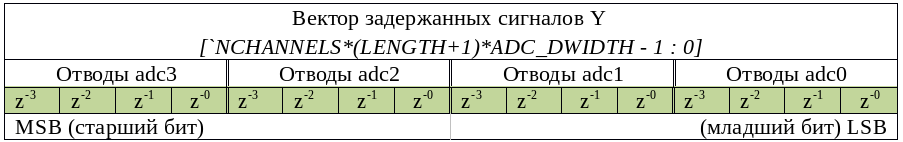
\includegraphics[width=12cm]{CRPA_CM_delay_line.png}
  \caption{Вектор задержанных отсчётов входных сигналов}
  \label{fig:CRPA_CM_delay_line}
\end{figure}

Далее рассчитывается матрица коэффициентов. Матрица имеет нижний треугольный
вид. Структура матрицы приведена на рис.~\ref{fig:CRPA_CM_struct}.
\begin{figure}
  \centering
  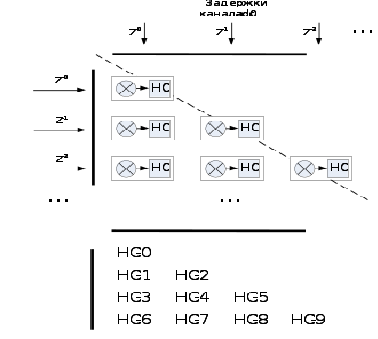
\includegraphics[width=8cm]{CRPA_CM_struct.png}
  \caption{Структура корреляционной матрицы}
  \label{fig:CRPA_CM_struct}
\end{figure}

Смещения указаны относительно начального адреса блока расчёта корреляционной матрицы
\texttt{CRPA\_CM} (см. разд. \ref{sec:commons}), равного 0x5000.

Расположение коэффициентов зависит от параметров реализованного фильтра
(см. \ref{sec:CRPA_PARAMS}): NF\_TIME --- количества отводов по времени и NF\_CHAN ---
количества входов блока помехоподавления.

Каждый коэффициент представляет собой действительное целое число со знаком.

\begin{longtable}{|c|p{3.5cm}|p{5cm}|p{4cm}|}
\hline
\textbf{Смещение} & \textbf{Название} & \textbf{Описание} & \textbf{Примечание} \\
% \hline
% 1 & 2 & 3 & 4  \\
% \hline\endfirsthead
% \hline
% 1 & 2 & 3 & 4 \\
% \hline\hline\endhead
% \hline
% \multicolumn{3}{c}{\textit{Продолжение на следующей странице}}
% \endfoot\hline\endlastfoot
\hline
0x00  (0x00) & CRPA\_CM\_R\_0\_0  & Элемент матрицы 0, 0 &  \\
\hline
0x04  (0x01) & CRPA\_CM\_R\_1\_0  & Элемент матрицы 1, 0 &  \\
\hline
0x08  (0x02) & CRPA\_CM\_R\_1\_1  & Элемент матрицы 1, 1 &  \\
\hline
\multicolumn{4}{|l|}{...} \\
\hline
0xXX  (0xYY) & CRPA\_CM\_R\_I\_J  & Элемент матрицы I, J &  \\
\hline
\multicolumn{4}{|l|}{...} \\
\hline
0x83C (0x20F) & CRPA\_CM\_R\_31\_31& Элемент матрицы 31, 31 & при $NF\_TIME=4$, $NF\_CHAN=8$ \\
\hline
\end{longtable}

% Local variables: 
% TeX-auto-local:"../../../pdf"
% TeX-master: "Correlator_title"
% End:
